\documentclass[a4paper, 11pt]{scrartcl}

% font, language
\usepackage[utf8]{inputenc}
\usepackage[T1]{fontenc}
\usepackage{lmodern}

\usepackage{float}
\usepackage{longtable}

% quoting
\usepackage{quoting, xparse}
\usepackage[hyphens]{url}

\usepackage[toc,page]{appendix}

% highliting
\usepackage{color,soul}

\usepackage[dvipsnames]{xcolor}

\usepackage{svg}
% \usepackage{ctable} % for \specialrule command
\usepackage{tabularx}

\NewDocumentCommand{\bywhom}{m}{% the Bourbaki trick
  {\nobreak\hfill\penalty50\hskip1em\null\nobreak
   \hfill\mbox{\normalfont(#1)}%
   \parfillskip=0pt \finalhyphendemerits=0 \par}%
}

\NewDocumentEnvironment{pquotation}{m}
  {\begin{quoting}[
     indentfirst=true,
     leftmargin=\parindent,
     rightmargin=\parindent]\itshape}
  {\bywhom{#1}\end{quoting}}

\usepackage{todonotes}
\usepackage{caption}
\newcommand{\source}[1]{\caption*{\hfill Source: {#1}} }

\usepackage{fontspec}
\setmainfont{Latin Modern Roman}

\usepackage{polyglossia}
\setmainlanguage[babelshorthands=true]{german}
\setdefaultlanguage[spelling=new]{german}
\usepackage[autostyle]{csquotes}
\MakeAutoQuote{»}{«}

\usepackage{enumitem}

% graphics
\usepackage{graphicx}
\graphicspath{ {images/} }

% code highlighting
\usepackage{listings}
\usepackage{color}
%\lstset{ % General setup for the package
%	language=java
%}

\lstset{
	%basicstyle=\scriptsize\sffamily\color{black},
	frame=single,
	numbers=left,
	numbersep=5pt,
	numberstyle=\tiny\color{gray},
	showspaces=false,
	showstringspaces=false,
	tabsize=1
}

\usepackage{listings}
\lstdefinelanguage{Kotlin}{
	comment=[l]{//},
	commentstyle={\color{gray}\ttfamily},
	emph={delegate, filter, first, firstOrNull, forEach, lazy, map, mapNotNull, println, return@},
	emphstyle={\color{OrangeRed}},
	identifierstyle=\color{black},
	keywords={abstract, actual, as, as?, break, by, class, companion, continue, data, do, dynamic, else, enum, expect, false, final, for, fun, get, if, import, in, interface, internal, is, null, object, override, package, private, public, return, set, super, suspend, this, throw, true, try, typealias, val, var, vararg, when, where, while},
	keywordstyle={\color{NavyBlue}\bfseries},
	morecomment=[s]{/*}{*/},
	morestring=[b]",
	morestring=[s]{"""*}{*"""},
	ndkeywords={@Deprecated, @JvmField, @JvmName, @JvmOverloads, @JvmStatic, @JvmSynthetic, Array, Byte, Double, Float, Int, Integer, Iterable, Long, Runnable, Short, String},
	ndkeywordstyle={\color{BurntOrange}\bfseries},
	sensitive=true,
	stringstyle={\color{ForestGreen}\ttfamily},
}

% toc depth
\setcounter{tocdepth}{4}
\setcounter{secnumdepth}{4}

% bib
\usepackage[
	backend=biber,
	sorting=none
]{biblatex}

\addbibresource{references/references.bib}
\usepackage{hyperref}
\usepackage{xcolor}
\hypersetup{
	colorlinks,
	linkcolor={red!0!black},
	citecolor={blue!70!black},
	urlcolor={blue!70!black}
}

\usepackage{enumitem}
\setlist[enumerate]{label*=\arabic*.}

% title, author
\title{Bachelor-Thesis}
\author{Roman Quistler}

\begin{document}
	
	
	
	% \begin{titlepage}
	\centering
	
\includegraphics[width=0.30\textwidth]{hsb_logo.png}
	\par\vspace{1cm}
	{\scshape\LARGE Hochschule Bremen \par}
	\vspace{1cm}
	{\scshape\Large Bachelorarbeit  \par}
	\vspace{1.5cm}
	{\LARGE\bfseries Entwicklung eines Model-View-Intent Framework für die Plattform Android\par}
	\vspace{0.5cm}
	{\normalsize\itshape Medieninformatik B.Sc. \par}
	\vspace{2cm}
	{\Large\itshape Roman Quistler \par}
	\vfill
	\vfill
	{\large\today\par}
\end{titlepage}
	
	\pagenumbering{gobble}
	\newpage
	\tableofcontents
	\newpage
	\pagenumbering{arabic}
	
	\newpage
	
	\section{Einleitung}
\label{sec:einleitung}

Bis zum Jahre 1973 und der Entwicklung des ersten Eingabegerätes mit Graphischer Oberfläche (GUI) (Xerox Alto \cite{xeroxAlto}) erfolgte die Interaktion mit einem Computer im Wesentlichen über eine Konsole. Dies reduzierte die Ein- und Ausgabe eines Programms auf rein textuelle Elemente. Seither hat sich viel getan: Die Erschaffung des Internets leitet den Beginn von Webseiten ein, welche von einer anfänglich statischen Ausprägung zu der heutigen dynamisch und komplexen wuchsen. Dazu gesellten sich im Laufe der Zeit mobile Endgeräte - zu Beginn bestückt mit Tasten für die Eingabe, sowie einem primitiven Bildschirm für die Anzeige finden sich heutzutage vorwiegend leistungsfähige, auf einem kapazitiven Touchscreen basierende Smartphones wieder. Hierbei ist über die Jahre der Funktionsumfang von Betriebssystem und Applikationen im Allgemeinen gestiegen.

\subsection{Problemfeld}
\label{subsec:problemfeld}
Die Herausforderung für einen Entwickler ist es, die Nutzerschnittstelle (auch: »Presenation Layer« \cite{presentationLayerpatternsOfEnterpriseApplicationArchitectureMartinFowler}),
innerhalb einer »Drei-Schichtenarchitektur«
\cite{threeTierArchitectureDonaldWolfe2013}
sinnvoll aufzubauen und dabei die Modellierung und Verwaltung des Zustandes innerhalb einer Applikation zu berücksichtigen. Hierfür müssen auch externe Vorkommnisse wie bspw.. die Aktualisierung der zugrundeliegenden Datenbank miteinbezogen werden.
\\\\
Da diese Problematik nicht erst seit kurzem sondern seit vielen Jahren besteht, wurden hierfür bereits unterschiedliche Ansätze entwickelt. Diese spiegeln sich in sogenannten Architekturmuster wieder und bieten ein Mittel, den »Presentation Layer« sinnvoll zu organisieren.
\\\\
Zu diesen Architekturmuster hat sich im Jahre 2015 ein neues hinzugesellt: »Model-View-Intent (MVI)«. Es besitzt bereits bekannte Herangehensweisen, setzt jedoch auch auf neue Ideen. Zu Beginn kam es ausschließlich in der Entwicklung von Webanwendungen zum Einsatz, bis es mit etwas Verzögerung auch in der (nativen) Android Entwicklung Einzug hielt. Wie es meist der Fall ist wenn neue Wege beschritten werden, ergibt sich viel Ungeklärtes. Dieses wächst wenn zusätzlich eine Wechsel der Plattform vorgenommenen, welche trotz Gemeinsamkeiten erhebliche Unterschiede und aufweist.
\\\\
Ist ein Entwickler an einem Einsatz von MVI interessiert, so ergeben sie für ihn gewisse, wenn auch übliche Hindernisse: Wie lassen sie die jeweiligen Komponenten umsetzten? Wie gut lassen sich Implementierungen für eine Plattform auf eine andere, seine Übertragen? Inwieweit müssen Eigenheit beachtet werden?  

\subsection{Ziel der Arbeit}
\label{subsec:ziel-der-arbeit}
Mit der Arbeit wird das Ziel verfolgt, das Architekturmuster MVI zu untersuchen, besser zu verstehen und im Kontext Android ein Framework zu schaffen.
\\
Es sollen Eigenheiten der Plattform, sowie allgemeine Probleme ausgemacht werden die für den Einsatz von MVI in Android relevant sind. Dazu müssen bereits bestehende Lösung evaluiert und vorhandene Problematiken aufgezeigt werden. Auf Basis der gewonnenen Erkenntnisse soll daraufhin ein kleines und dogmatisches Framework entwickelt werden. Die Absicht ist dem Anwender alle nötigen Komponenten zu Realisierung von MVI zur Verfügung zu stellen und eine klare Struktur vorzugeben. Dabei soll der Aufwand seitens des Nutzers möglichst gering gehalten werden.

\subsection{Aufbau der Arbeit}
\label{subsec:aufbau-der-arbeit}
Im ersten Schritt werden die nötigen Grundlagen für ein besserer Verständnis von MVI geklärt. Dazu gehören spezielle Paradigmen der Programmierung als auch vorausgegangene Konzepte und Bibliotheken.
\\\\
Ist dies Vollbracht so wird im nächsten Schritt MVI mit all seinen Komponenten genau beschrieben. Es wird auch versucht, die Gründe für die Entstehung von MVI zu finden und zu erläutern.
\\\\
Daraufhin werden die Funktionalen und Nichtfunktionalen Anforderung für das zu entwickelnde Framework aufgelistet und näher ausgeführt. Hierbei soll Erkennbar ein, worauf der Fokus liegt und was als Optional eingestuft wird. 
\\\\
Im weiteren Fortgang wird mit diesen Anforderung und den zuvor erworbenen Kenntnissen das Framework und seine individuellen Komponenten konzipiert. Jeder dieser wird ausführlich beleuchtet und ihre Funktion dargelegt. Auch die Zusammenhänge innerhalb des Frameworks werden aufgegriffen und erörtert.
\\\\
Anschließend erfolgt die Implementation des Framework in Form eines Prototypen. Zuvor werden jedoch Grundlegende Entscheidungen und ihre Auswirkungen erläutert. 
\\\\
Als vorletzter Schritt werden die jeweiligen Anforderungen auf Basis des Prototypen ausgewertet. Es wird geschaut zu welchem Grad diese Erfüllt wurden und falls nicht, welche Gründe dies hat und wie es umgesetzt werden könnte. Außerdem sollen eventuelle Verbesserungen diskutiert werden.
\\\\
Zum Schluss wird die Arbeit und ihr Ergebnis zusammengefasst und ein Ausblick gegeben.

	\newpage
	
	\section{Grundlagen}
\label{sec:grundlagen}

In diesem Kapitel gilt es zu klären, auf welchen Grundlagen, Ideen und Konzepten Model-View-Intent beruht, wie diese miteinander fungieren und weshalb sie als Inspiration dienten.

\subsection{Unidirektionaler Datenfluss und der Zustand: Flux, Redux und Elm}

In einer Applikation existieren grundsätzlich zwei Komponenten: Eine, die der Nutzer wahrnehmen kann und eine, die für ihn unsichtbar bleibt. Bei ersterer handelt es sich meist um das, was der Nutzer(auf dem Bildschirm) sieht - die sogenannte »View«. Die zweite Komponente beschreibt die Ebene, welche das Geschehen observiert, darauf reagiert und den weiteren Verlauft (zum größten Teil) kontrolliert. Sie kann unter anderem als »Controller« betitelt werden.
\\
\\
Ein weiterer, essentieller Aspekt einer Anwendung ist ihr Zustand. Dieser kann sich aus mehreren Teilen zusammensetzten:
\begin{itemize}
	\item Alles was der Nutzer sieht
	\item Daten die über das Netzwerk geladen werden
	\item Standort des Nutzer
	\item Fehler die auftreten
	\item \dots
\end{itemize}
Der Zustand in dem sich eine Applikation befindet kann hierbei von beiden Seiten modifiziert und beobachtet werden. Ist dies der Fall, so handelt es sich um einen bidirektionalen Datenfluss. Bei dieser Variante entsteht die eventuelle Gefahr von kaskadierenden Updates (ein Objekt verändert ein anderes, welches wiederum eine Veränderung bei einem weiteren herbeiführt usw.) als auch in einen unvorhersehbaren Datenfluss zu geraten: Es wird schwer, den Fluss der Daten nachzuvollziehen. Des weiteren muss immer überprüft und sichergestellt werden, dass »View« und »Controller« synchronisiert sind, da beide den globalen Zustand darstellen. Schlussendlich verliert man zusätzlich die Fähigkeit zu entscheiden, wann und and welcher Stelle der Zustand manipuliert wird.
\\
\\
Ein anderer Ansatz ist, den Datenfluss in eine Richtung zu beschränken und ihn damit unidirektional
\cite{unidirectionalDataFlowFluxArchitectureIlyGelman2017, unidirectionalDataFlowTheCompleteReduxBookIlyGelman2017}
operieren zu lassen. Diese Variante erfreut sich an zunehmender Popularität seit der Bekanntmachung der »Flux«
\cite{fluxArchitectureAdamBoduch}
Architektur im Jahre 2015 von Facebook.
\cite{fluxAnnouncementYoutube}

\subsubsection{Flux}
Für die Einhaltung und Umsetzung eines unidirektionalen Datenfluss und der Verwaltung des Zustands bedient sich »Flux« bei zwei fundamentalen Konzepten: Der Zustand innerhalb einer Applikation wird als »single source of truth (SSOT)« angesehen und darf keine direkte Änderung erfahren. Um dies zu Gewährleisten finden sich mehrere Komponenten in »Flux« wieder:
\\
\\
\textbf{Action}: Eine Aktion beschreibt ein Ereignis, welches unter anderem vom Nutzer ausgelöst werden kann. Sie geben vor, wie mit der Anwendung interagiert wird. Jeder dieser Aktionen wird dabei ein Typ zugewiesen. Insgesamt sollte eine Aktion semantisch und deskriptiv bezüglich der Intention sein. Des weiteren können zusätzliche Attribute an eine Aktion gebunden werden.
\\
\begin{lstlisting}[frame=single, language=Java]
{
 type: ActionTypes.INCREMENT,
 by: 2
}
\end{lstlisting}
\bigskip
\textbf{Dispatcher}: Er ist für die Entgegennahme und Verteilung einer Aktion an sogenannte »Stores« zuständig. Diese haben die Möglichkeit sich beim ihm zu registrieren. Er besitzt die wichtige Eigenschaft der sequentiellen Verarbeitung, d.h., dass er zu jedem Zeitpunkt nur eine »Action« weiterreicht. Sämtliche »Stores« werden über alle Aktionen unterrichtet.
\\
\\
\textbf{Store}: Hier befinden sich die Daten, welche einen Teil des globalen Zustands einer Anwendung ausmachen. Die einzige Möglichkeit für eine Veränderung der dort hinterlegten Daten besteht durch ein Reaktion auf eine, vom »Dispatcher« kommenden, Aktion. Bei jeder Modifikation der Daten erfolgt die Aussendung eines Events an eine »View«, das die Veränderung mitteilt.
Ebenso findet sich hier ein Part der Anwendungslogik.
\\
\\
\textbf{View}: Die View ist für die Anzeige und Eingabe von Daten zuständig - sie ist die für den Nutzer sichtbare Komponente, mit welcher dieser interagiert. Ihre Daten erhält sie von einem »Store«, diesen sie abonniert und auf Änderungsereignisse hört. Erhält sie vom »Store« ein solches Änderungsereignis, so kann sie die neuen Daten abrufen und sich selbst aktualisieren. Der View ist es nicht gestattet, den Zustand direkt zu verändern. Stattdessen generiert sie eine Aktion schickt diese an den Dispatcher.
\\
Ein Beispielhafter Ablauf bei einer Anwendung die einen Wert erhöht oder verringert kann wie folgt aussehen:
\begin{enumerate}
	\item Die View bekommt einem Store zugewiesen, welcher für das inkre- und dekrementieren der angezeigten Zahl verantwortlich ist.
	\item Sie erhält die Anfangszahl und stellt diese in einem leserlichen Format/einer Ansicht dar, welches es dem Nutzer ermöglicht, damit zu interagieren.
	\item Betätigt dieser einer der Knöpfe welche die dargestellte Zahl verändern, so wird eine Action erstellt und an Dispatcher geschickt.
	\item Dieser wiederum informiert alle Stores.Information
	\item Jener Store der für die Verarbeitung dieser Aktion verantwortlich ist, modifiziert die Zahl in seiner internen Datenstruktur und kommuniziert dies über ein Änderungsereignis
	\item Diejenige View, welche auf Änderungsereignisse diesen Ursprungs lauscht, erhält die Daten und aktualisiert sich dementsprechend. 
\end{enumerate}

\begin{figure}[ht]
	\centering
	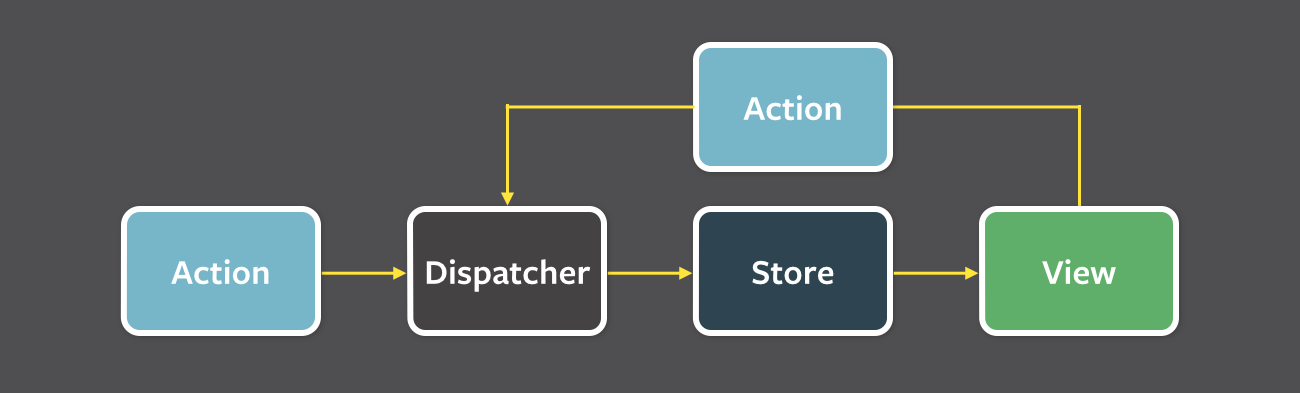
\includegraphics[height=0.25\textwidth]{./images/flux-flow}
	\caption{Datenfluss in der Flux Architektur}
	\label{fig:datenflussFlux}
\end{figure}

Anhand Abbildung \ref{fig:datenflussFlux} wird der unidirektionale Datenfluss deutlich erkennbar:
\begin{enumerate}
	\item Die View schickt eine Aktion an den Dispatcher.
	\item Dieser leitet diese an alle Stores weiter.
	\item Der Store verarbeitet die Daten und informiert die View.
\end{enumerate}
\bigskip
Insgesamt liefert Flux mit diesen Komponenten eine Möglichkeit, einen unidirektionalen Fluss herzustellen und die Verwaltung des Zustands einer Applikation zu vereinfachen.
\subsubsection{Redux}
Bei Redux handelt sich um eine JavaScript Bibliothek (und kein Framework) welche ihre Inspiration aus Flux und Elm bezieht. Sie wurde im Jahre 2015 von Dan Abramov und Andrew Clark ins Leben gerufen.
\cite{reduxIntroduction}
Auch hier nimm der direktionale Datenfluss eine wesentliche Rolle ein.
\\
\\
Die Bibliothek kann als eine vereinfachte Form von Flux verstanden werden, welche gewisse Elemente und Ansätze übernimmt, aber auch streicht bzw. ersetzt. Genau wie Flux existieren die bereits behandelten Actions, welche über wichtige Informationen für die spätere Veränderung des Zustands verfügen. Auch hier können diese ihren Ursprung in einer vom Nutzer getätigten Aktion haben. Wird eine Aktion ausgeführt, so spricht man von einer Versendung einer Aktion. Dieser Versand findet nur dann statt, wenn man die Intention verfolgt, den Zustand zu ändern. Sie gelangt zu einem sogenannten "Reducer". Hier findet sich der erste Grundlegende Unterschied zu Flux.
\\
\\
Ein "Reducer" ist für sich genommen eine einfache Funktion, die bei gleicher Eingabe die immer gleiche Ausgabe erzeugt. Sie ist dabei frei von sogenannten Seiteneffekten und wird als "pure" bezeichnet. Im Falle eines "Reducers" erwartet dieser die vorher erzeugte Aktion und den globalen, derzeitigen Zustand der Anwendung. Sein Aufgabe ist es, aus der Kombination dieser einen neuen Zustand zu generieren. Hierfür wird die Aktion, basierend auf ihrem Typ und eventuellen Inhalt, ausgewertet und der Zustand dementsprechend angepasst. Dabei ist zu beachten, dass keine direkte Manipulation des Zustands möglich ist, stattdessen wird ein komplett neuer Zustand zurückgegeben. Diese Eigenschaft der Unveränderbarkeit wird gemeinhin als "Immutability" erfasst.
\\
\begin{lstlisting}[frame=single, language=Java]
(previousState, action) => newState
\end{lstlisting}
\ \\
Das Verbindungsstück zwischen einer Aktion und dem Reducer bildet der Store. Dieser existiert im Gegensatz zu Flux nur ein einziges Mal (und mit auch der Zustand) und ist für die Verwaltung des Zustands verantwortlich. Er übernimmt zugleich auch die Rolle des Dispatchers, wie er in Flux vorkommt, und verteilt die Akionen an alle Reducer weiter. Der aus dem diesen Prozess hervorgehende, neue Zustand wird im Store hinterlegt. Dieses Ereignis wird ebenfalls seitens der View observiert, welche im Anschluss die nötigen Aktualisierungen an der Ansicht vornimmt.
Am Ende lässt sich der gesamte Fluss wie folgt darstellen:
\\
\begin{lstlisting}[frame=single, language=Java]
View -> Action -> Reducer(s) -> Store -> View
\end{lstlisting}
\bigskip
Neben Redux existieren in der JavaScript Welt noch weitere Bibliotheken, die entweder eine Abwandlungen von Flux darstellen oder aber neue Konzepte implementieren. Jedoch verfolgen dabei alle eine ähnliches Ziel: Ein unidirektionaler Datenfluss und die (zentrierte) Verwaltung des Zustands einer Anwendung.

\subsubsection{Elm}
Bei Flux und Redux handelt es sich jeweils um Bibliotheken die innerhalb einer Anwendung verwendet werden können. Eine weitere Herangehensweise ist die Verankerung solcher Konzepte in der Programmiersprache selbst. Dies findet man z.B. in
der Programmiersprache Elm
\cite{elmIntroduction}
wieder. Elm besitze eine in die Sprache integrierte Architektur die den einfach Namen "The Elm Architecture" 
\cite{theElmArchitecture}
trägt. Eine andere Variante lautet: Model-View-Update. Anhand dessen lassen sich bereits die Kern-Komponenten der Entwurfsmusters erahnen.
\\
\\
\textbf{Model:} Das Model repräsentiert den Zustand der Applikation als eine simple Datenstruktur.
\\
\textbf{View:} Die View ist eine Funktion, welche aus einem Model HTML code generiert. Ebenfalls wie in Flux wird kommt auch hier das Konzept von "pure functions" zum tragen: Die gleiche Eingabe erzeugt die gleich Ausgabe - ohne Ausnahme.
\subsection{Funktionale Programmierung}
Im Verlaufe der Kapitel wurden bereits Begriffe wie eine "reine" Funktion (pure functions) oder die Unveränderlichkeit (Immutibilty) einen Datenstruktur angesprochen. Diese Konzepte zählen zu einem Programmierparadigma, welches in den letzten Jahren auch an Bedeutung in Sprachen wie Java gewonnen hat
\cite{javaFunctionalProgramming}
: Funktionale Programmierung.
\\
\\
In der häufig imperativen, Objektorientierte Programmierung wie sie in Java oder auch C\# anzutreffen ist, machen Klassen und
die Mutation (in möglicher Abhängigkeit von gewissen Konditionen) solcher den Hauptbestandteil des Quellcodes aus. Dabei ist zu beachten, dass die funktionale Programmierung die Objektorientierte nicht zwingenden ausschließt, sondern lediglich in eingeschränkter Form nutzt.
Eine Implementierung in Java welche Beispielweise den Name eines Nutzer Objekts ändert, könnte wie folgt aussehen:
\begin{lstlisting}[frame=single, language=Java]
public User changeUserName(String newUserName, User currentUser){
 if(newUserName != null){
  currentUser.name = newName
		
  System.out.println("Changed user name to: " + newUserName)	
 }
	
 return currentUser
}
\end{lstlisting}

	
	\newpage
	
	\section{Model-View-Intent}
\label{sec:model-view-intent}
In diesem Kapitel wird MVI unter die Lupe genommen und genauer beschrieben.

\subsection{Vorausgegangene Architekturmuster}
Hier werden in kurzer Ausführung die bekanntesten Architekturmuster neben Model-View-Intent beschrieben.

\subsubsection{Model-View-Controller}
Mode-View-Controller oder auch MVC ist eines der ältesten Architekturmuster und wurde im Jahre 1979 von Trygve Reenskaug veröffentlicht.
\cite{theModelViewEditorTrygveReenskaug1979, modelsViewsControllersTrygveReenskaug1979}
Es besteht aus drei Komponenten mit folgenden Funktionen:
\begin{itemize}
	\item \textbf{Model}: Es beschreibt den Zustand der Anwendung durch das Festhalten von Daten und aktualisiert informiert die View über Veränderungen. (View)
	\item \textbf{View}: Sie ist für die Darstellung des UI zuständig und aktualisiert sich bei Änderungen im Model.
	\item \textbf{Controller}:  Er kontrolliert die beiden anderen Komponenten und enthält möglicherweise weitere (Business) Logik. Dafür nimmt Ereignisse aus der View bzw. vom Nutzer entgegen und manipuliert daraufhin das Model oder die View direkt. 
\end{itemize}
\begin{figure}[ht]
	\centering
	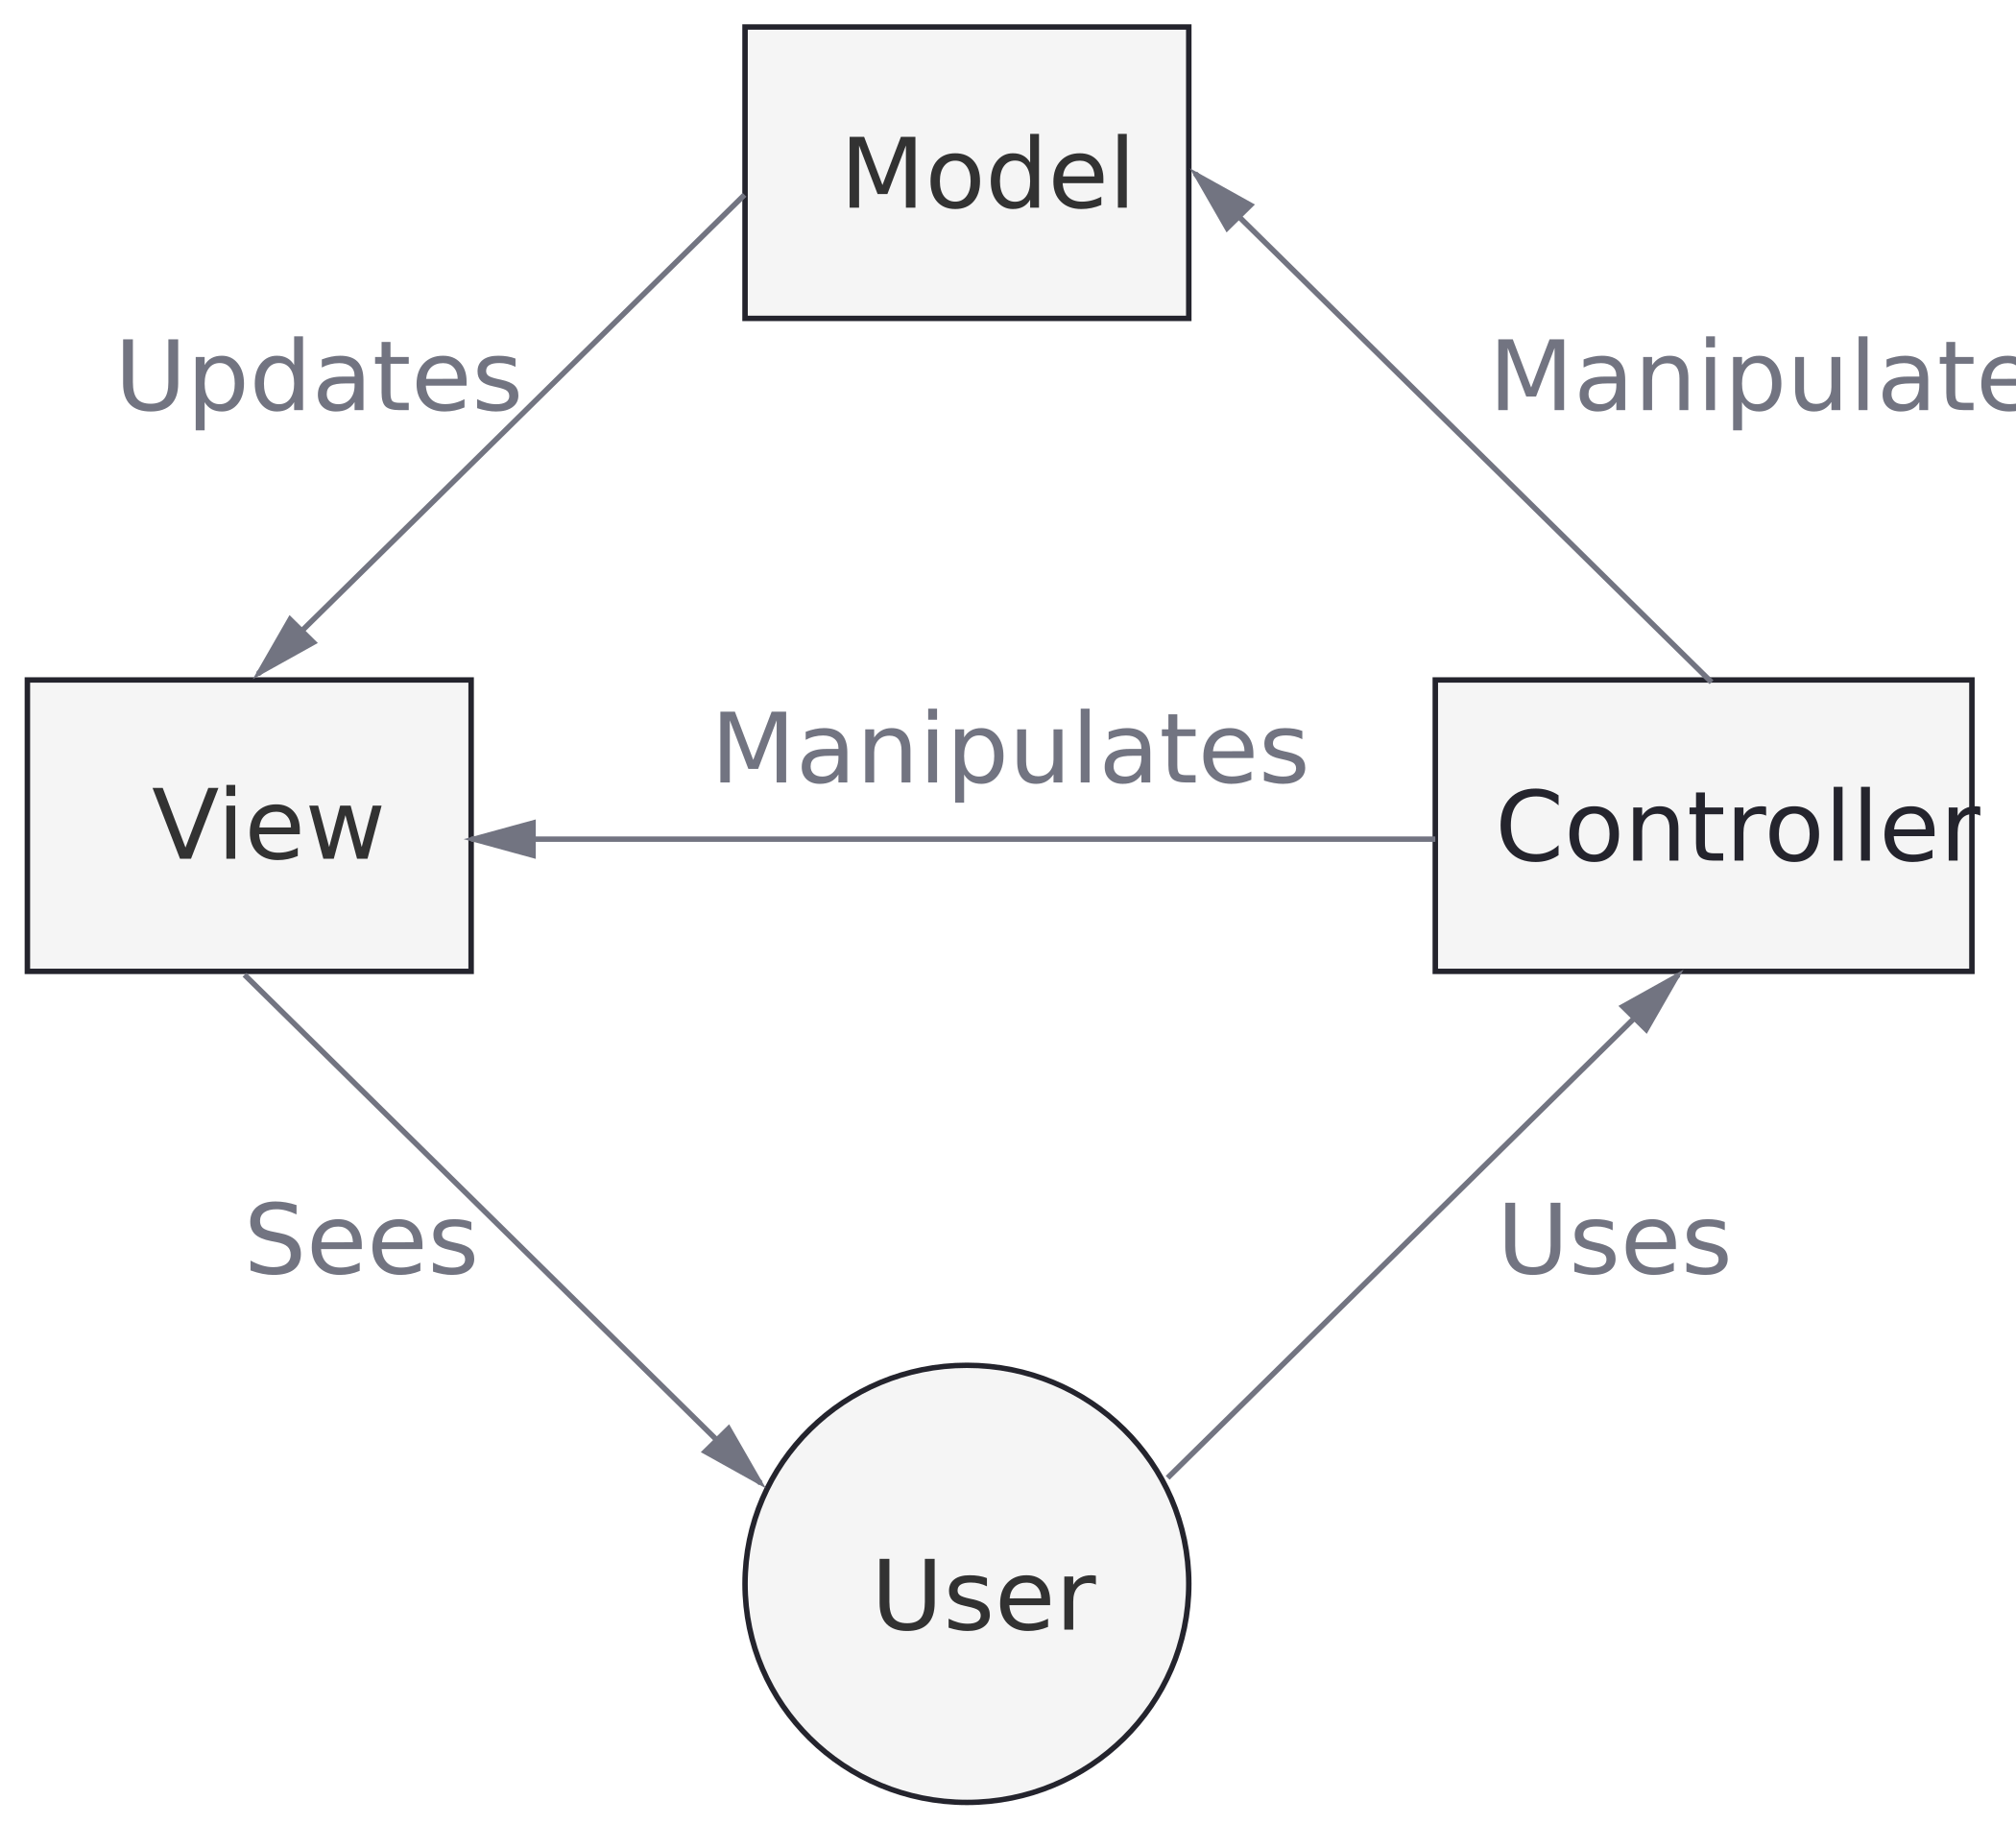
\includegraphics[height=0.5\textwidth]{./images/mvc-diagram.png}
	\caption{Model-View-Controller}
	\label{fig:mvc}
\end{figure}
\clearpage

\subsubsection{Mode-View-Presenter}
Das nächste im Bunde ist Model-View-Presenter (MVP) aus dem Jahre 1996.
\cite{modelViewPresenterTheTaligentMikePotel1996, modelViewPresenterMartinFowler2006}

\subsubsection{Model-View-ViewModel}

\subsection{Historie \& Grundlegendes}
Model-View-Intent (MVI) ist eine weiteres Entfursmuster, welches der Feder von André (Medeiros) Staltz entstammt. Er stellte dieses auf einer Javascript Konferenz im Jahre 2015 vor
\cite{modelViewIntentIntroduction}. Es gehört damit zu den jüngsten seiner Art.
Seine ursprüngliche Anwendung fand es in dem ebenfalls von André Staltz geschaffenen Framework CycleJs, hat seit der Artikelreihe von Hannes Dorfmann in 2016
\cite{modelViewIntentOnAndroidHannesDorfmann2016}
aber auch den Sprung in die Welt von Android vollbracht. MVI bezieht den Großteil seines Design aus den hier bereits vorstellten Ideen und Konzepten. Das erste Ziel ist, ähnlich wie bei MVC, Informationen zwischen zwei Welten zu übersetzten: der des digitalen Bereichs des Computers und des mentalen Modells des Benutzers. Oder anders formuliert: Das Programm muss verstehen, was der Nutzer im Sinn hat.
Der zweite, zentrale Punkt von MVI besteht in der Handhabung des Zustands der Anwendung. Hierfür ist zu klären, was genau der Zustand inne hat.
\\
\\
MVI betrachtet dafür die Interaktion zwischen einem Nutzer und Programm als einen Kreis(lauf). Betätigt der Nutzer bswp. einen Knopf, sein Output, so gestaltet sich dieser als Input für das Programm. Dieses wiederum erzeugt einen Output (z.B. eine Meldung), welcher zum Input des Nutzers wird (hier: lesen).
\begin{figure}[ht]
	\centering
	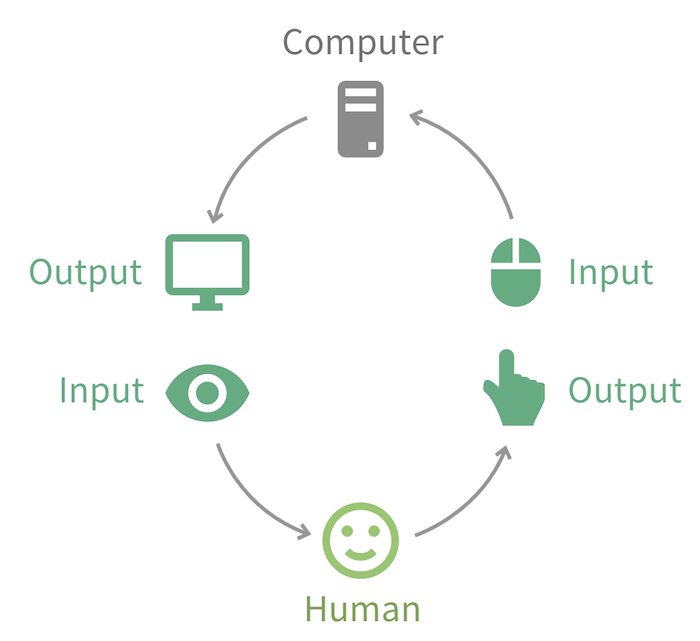
\includegraphics[height=0.5\textwidth]{./images/mvi-cycle}
	\caption{Nutzer und Computer als Input und Output}
	\caption*{Source: https://cycle.js.org/dialogue.html}
	\label{fig:userComputerInputOutput}
\end{figure}
\\
Die Grundprinzipien für den Aufbau der Architektur entspringen dabei dem beschriebenen, originalem Model-View-Controller. Das, was MVC jedoch inkompatibel für die von MVI vorhergesehenen Prozesse macht, ist die Tatsache, das der Controller proaktiv ist. Dies bedeutet, dass der Controller selbstbestimmt über das Model und View verfügen und diese direkt manipulieren kann. Zwangsläufig wissen die jeweiligen Komponenten auch, von welchen Komponenten sie abhängig sind. Oder anders ausgedrückt: Eine Komponente deklariert, welche anderen Komponenten sie beeinflussen, anstatt dass andere Komponenten explizit aktualisiert werden (z.B. das Modell). Dabei wird das Prinzip des unidirektionale Datenfluss verletzt, welches auch in MVI strikt verfolgt wird. 
\\
\\
Um dieses unter anderem zu erreichen, setzt MVI zusätzlich auf Reaktive Programmierung. Für MVI bedeutet reaktiv zu sein, dass jede Komponente ihre Abhängigkeiten beobachtet und auf Veränderungen dieser reagiert. Die drei Komponenten werden durch Observables repräsentiert, wobei der Output jeweils der Input einer anderen Komponente ist.

\subsection{Model, View \& Intent}
Fast noch wichtiger als der reaktive Ansatz ist zu verstehen, wie der Kreislauf in Figur \ref{fig:userComputerInputOutput} 
programmatisch etabliert werden kann. Betrachtet man diesen Kreis etwas genauer, so wird deutlich, dass auf einen Input immer ein Output folgt. Dieses Konzept findet man auch in der Mathematik wieder: Funktionen. Mit diesen lässt sich MVI wie folgt illustrieren:
\\
\\
\textbf{Intent}: Das I in MVI steht für Intent und stellt den Teil da, welches es von den anderen Entwurfsmustern unterscheidet. Das Ziel der Intent-Fuktion ist es, die Absicht des Nutzer im digitalen Kontext des Programms auszudrücken.
Ein Ereignis (oder Event), z.B. die Eingabe eines Buchstaben, kann hier der Input sein.
Der Output dieser Funktion (z.B. ein String) wird zum Input der nächsten:
\\
\\
\textbf{Model}: Die Model-Funktion nimmt das entgegen, was die Intent-Funktion produziert. Ihre Aufgabe liegt in der Verwaltung des Zustands: Sie verfügt über das Model. Sie kann daher durchaus als das zentrale Element in MVI bezeichnet werden. In Anbetracht der Tatsache, dass MVI sich als auf funktionaler Programmierung basierendes Muster versteht, ist das Model unveränderlich. Daraus ergibt sich zwangsläufig, dass für einen Zustandswechsel das Model kopiert und somit ein neues erzeugt werden muss. 
\\
Diese Funktion ist der einziges Teil des Programms, welche eine Zustandsveränderung hervorrufen kann und darf. Zusätzlich ist es der Ort, an dem auf die Business Logik der Anwendung zugegriffen wird.
\\
\\
\textbf{View}: Die View ist die letzte Funktion in der Kette, und ist zuständig für die visuelle Repräsentation des Models.
\newpage
Nimmt man alle drei Funktion zusammen, ergibt sich folgende Kette:
\begin{lstlisting}[caption={funktion}, xleftmargin=.3\textwidth, frame=false, numbers=none]
view(model(intent(input)))
\end{lstlisting}
Um den Sachverhalt zu verdeutlichten, kann dieses Beispiel in Form von pseudo-code herangezogen werden:
\begin{lstlisting}[caption={pseudo mvi implementation}, label={lst:pseudo-mvi}, language=Kotlin]
fun intent(text: String): Event {
	return EnteredTextEvent(text)
}

fun model(event: Event): Model {
	return when(event){
		is EnteredTextEvent -> {
			val newText = event.text.trim() // <-- business logic
			model.copy(text = newText) // <-- immtuable data structure
		}
	}
}

fun view(model: Model){
	textView.text = model.text 	
}

fun main(args : Array<String>) {
	view(model(intent("Hello World")))
}
\end{lstlisting}
Bei dieser Implementierung ist jedoch schnell ersichtlich, das es sich hierbei um keinen Kreis(lauf) handelt. Jede Funktion wird nur einmal aufgerufen. Es fehlt der reaktive Part, der MVI unter anderem ausmacht. Um diesen zu realisieren muss der Beispiel-Code wie folgt abgeändert werden:
\begin{lstlisting}[caption={pseudo mvi implementation},label={lst:pseudo-reactive-mvi},language=Kotlin]
// the obersvable from the textView gets passed as a parameter
fun intent(text: Observabkle<String>): Observable<Event> {
	text.map { text -> EnteredTextEvent(text) }
}

fun model(event:  Observable<Event>): Observable<Model> {
	event.map { event ->
		return when(event){
			is EnteredTextEvent -> {
			val newText = event.text.trim() // <-- business logic
			model.copy(text = newText) // <-- immtuable data structure
		}
	}	
}

fun view(model: Observable<Model>){
	// we subscribe to the model to listen for changes
	model.subscribe { model ->
		textView.text = model.text 	
	}	
}

fun main(args : Array<String>) {

	// this listens to arbitary text changes 
	val textChanges: Observable<String> = textView.changes()

	view(model(intent(textChanges))) 
}
\end{lstlisting}
Ein Punkt der in dieser Implementation noch offen bleibt, ist woher das Model kommt wie es verwaltet wird.

\subsection{Reducer}
Schaut man sich die Model-Funktion in Beispiel \ref{lst:pseudo-reactive-mvi} und ihren Inhalt genau an, so wird ein bestimmtes Muster bzw. ein sich wiederholender Ablauf erkennbar:
\\
\begin{enumerate}
	\item Die Funktion erhält ein Event 
	\item Die Funktion evaluiert das Event
	\item Die Funktion führt basierend auf dem Event (Business) Logik aus
	\item Die Funktion erzeugt ein neues Model
	\item Die Funktion gibt das neue Model zurück
\end{enumerate}
Der einzige Schritt der Fehlt, ist die Bereitstellung des derzeitigen oder des vorherigen Models. Hier kommt eine Komponente ins Spiel, die bereits in Kapitel \ref{subsec:redux} angesprochen wurde: der Reducer.
\subsection{Endlicher Automat}
Wenn der in der Model-Funktion ausgeführte Code eine neues Model hervorbringt, so bleibt der Zustand entweder der Gleiche oder er verändert sich. Unabhängig davon geht der Zustand in den selbigen oder in einen neuen Zustand über: es kommt zu einem sogenannten Zustandsübergang. Aber nicht nur das lässt sich aus dem gezeigten Beispiel ableiten; es sind noch weitere Schlussfolgerungen zulässig:
\\
\begin{itemize}
	\item Es gibt immer einen Anfangszustand bzw. Startzustand
	\item Es gibt eine endliche Anzahl von Zuständen
	\item Es gibt eine beliebe Menge von Endzuständen
	\item Es gibt immer nur einen Zustand, in dem sich die Anwendung befinden kann
\end{itemize}
\bigskip
Die oben genannten Punkte lassen sich anhand eines weiteren Beispiels besser erläutern: Man nehme an, dass sich auf einem Bildschirm ein Textfeld und ein dazugehöriger Knopf befindet. Das Textfeld ist anfänglich leer und der Knopf deaktiviert. Dieser kann nur aktiviert werden, wenn eine Eingabe im Textfeld erfolgt. Hiermit ist der Startzustand des Knopfs "deaktiviert" (z0). Gibt der Nutzer im Textfeld einen Text ein, so wird der Knopf aktiviert. Dieses Ereignis ist der bereits angeführte Zustandsübergang.
Gleichzeitig wird ein Endzustand erreicht (z1) - weitere Eingaben führen zu keinem neuem Zustand.
Die Beschreibungen z1 und z2 dienen hierbei als das Eingabealphabet und zeigen die Menge von potenziellen Ereignissen auf.
\begin{figure}[ht]
	\centering
	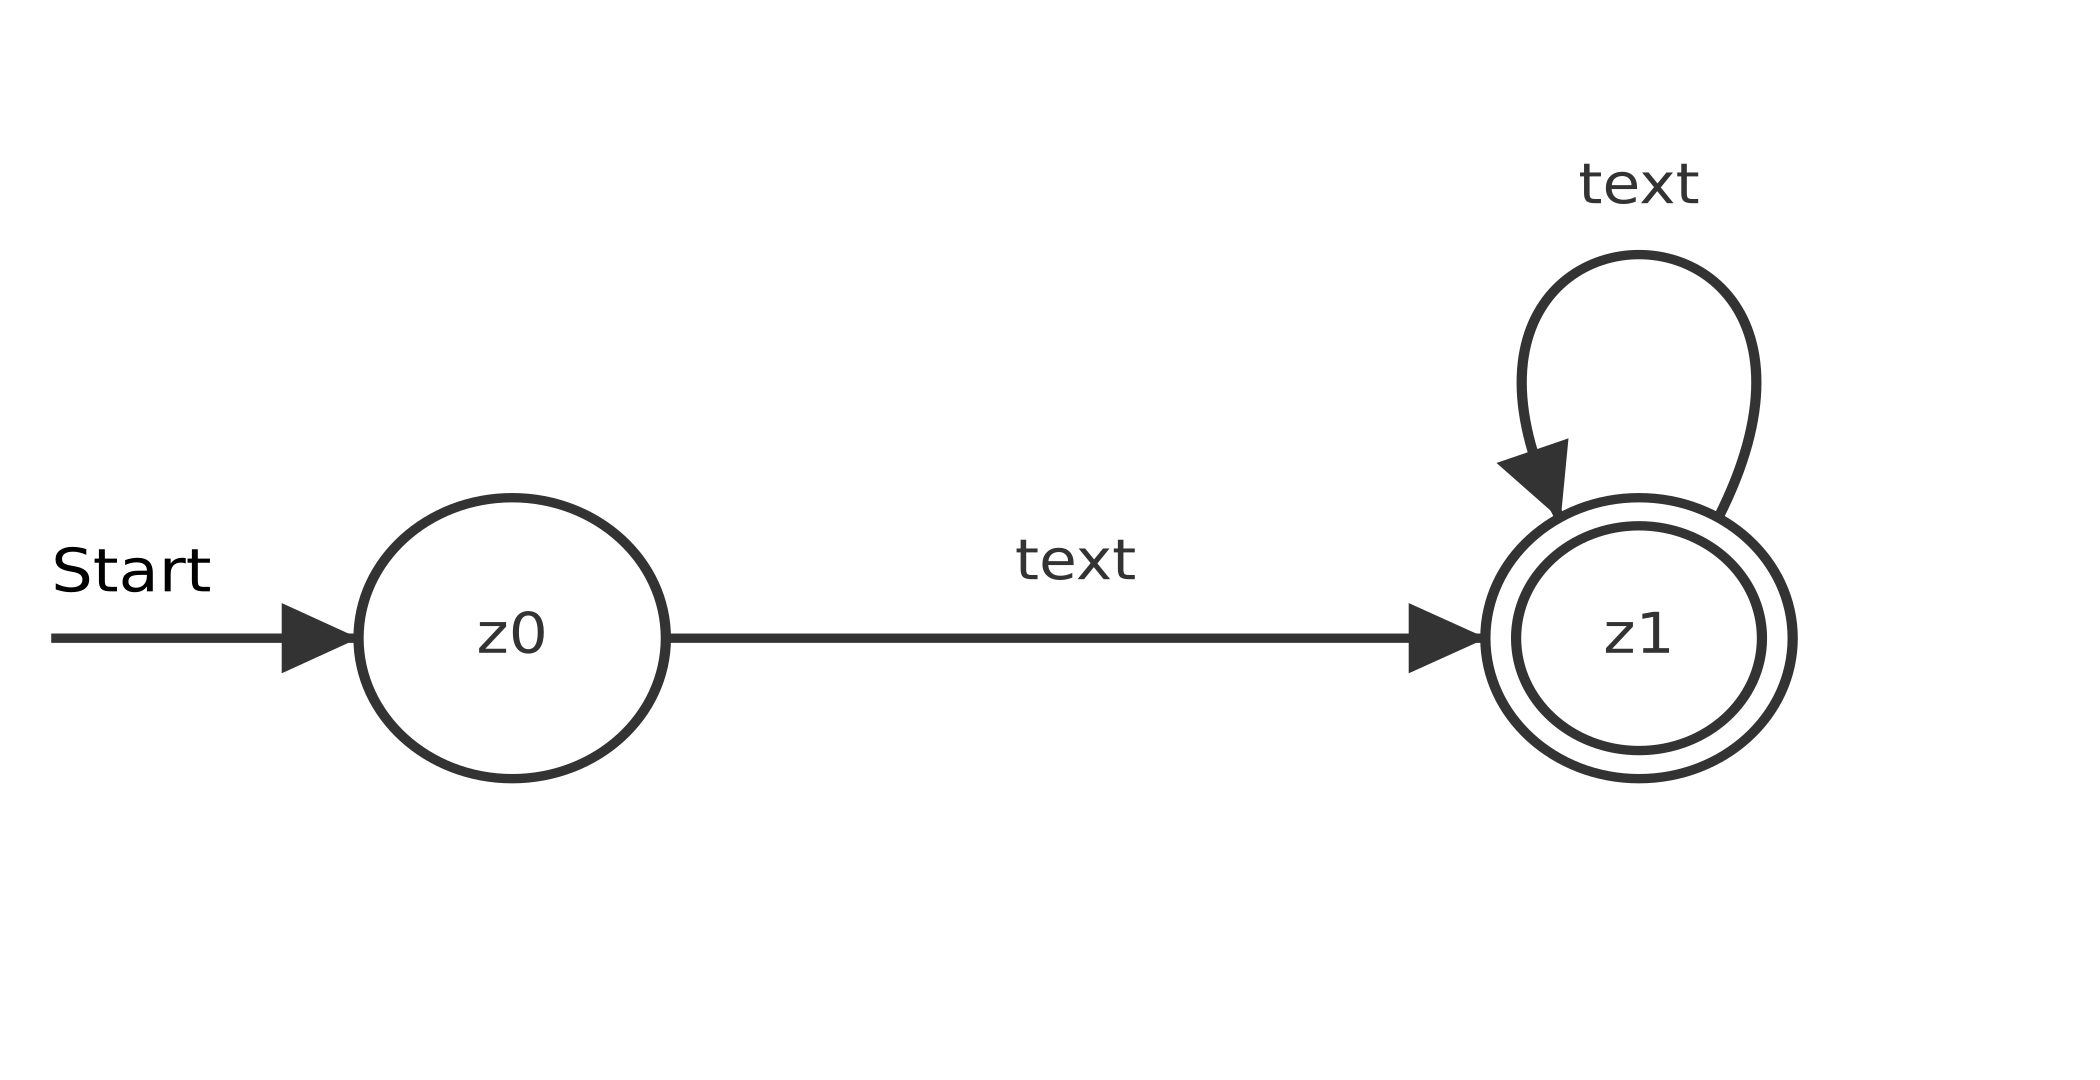
\includegraphics[height=0.35\textwidth]{./images/out}
	\caption{Endlicher Automat}
	\label{fig:endlicherAutomat}
\end{figure}
\\
Dieses Konzept ist in der Informatik bekannt als "Endliche Automaten". Ihr Ziel ist es, ein bestimmtes Verhalten (wie das obige) zu Modellieren und unter anderem visuell in Form von Abbildung
\ref{fig:endlicherAutomat} 
zu präsentieren.
	
	\newpage
	
	\section{Anforderungsanalyse}
\label{sec:anforderungsanalyse}

\subsection{Funktionale Anforderungen}
Die Funktionalen Anforderungen dienen dafür, um die genaue Funktionalität und das Verhalten eines Systems zu beschreiben. Es wird behandelt, was das System können soll und muss. Um dies besser abbilden zu können, werden die einzelnen Anforderungen einer Gewichtung unterzogen. Diese Gewichtung lässt sich in Form von "Muss","Soll" und "Kann" Anforderungen ausdrücken. Aufgrund des kleines Rahmens und Zeitfensters dieser Thesis wird sich im diesen Teil ausschließlich auf "Muss"-Anforderungen beschränkt, d.h. jene Funktionalität, welches das Framework erfüllen muss. Für die Übersichtlichkeit werden sämtliche Anforderungen nummeriert und mit dem Kürzel "FA" versehen.
\\
\\
\textbf{[FA01] Identifizieren von "Intents"}
\\
Dem Nutzer des Frameworks muss es möglich sein, die "Intents" seiner Anwendung eindeutig zu markieren.
\\
\\



	
	\newpage
	
	\section{Design \& Konzept}
\label{sec:design-und-konzept}
In diesem Kapitel ...

\subsection{Grundlegende Designentscheidungen}
Bevor auf Entscheidungen eingegangen wird ...

\subsubsection{Android als Plattform}
Das Framework richtet sich ausschließlich an Entwickler die Applikationen für die Plattform Android entwickeln. Es ist damit nicht kompatibel zu iOS, dem Web oder Serverseitigen Anwendungen. Die Spezialisierung lässt es jedoch zu, besser auf mögliche Eigenheiten der Plattform einzugehen. Ein weiterer Grund für diese Entscheidung stellt die Tatsache dar, dass MVI seinen Anfang in der Entwickelung von Webseiten fand und es sich im Fall Android um einen Nachzügler handelt.

\subsubsection{Framework}
Warum Framwork? Besonderheiten...

\subsubsection{Kotlin als Programmiersprache}
Die Applikationen in Android und das Android-SDK selbst sind bis vor wenigen Jahren fast ausschließlich in der Sprache Java entwickelt wurden. Seit der Google I/0 2017 gehört jedoch eine weitere Sprache zu den offiziell unterstützen:  Kotlin. Sie wird von dem Unternehmen Jetbrains entwickelt, die untere anderem die Entwicklungsumgebung Intellij für Java produzieren. Dieses bildet auch die Grundlage für Android Studio.
Kotlin hat in den letzten Jahren an Bodenhaftung gewonnen und findet auch intern bei Google Verwendung.
\\
Die Sprache wird als statisch typisierte, objektorientierte Programmiersprache bezeichnet und verfügt über eine hohe Interoperabilität zu Java. Dies bedeutet, dass innerhalb eines in Java geschriebenen Programms ohne viel Aufwand Kotlin genutzt werden kann. Dies ist ein wichtiger Faktor für die immer weiter ansteigende Beliebtheit, da es eine einfache Integration und bisherige Projekte gestattet. 
Kotlin bringt ein verbesserte Syntax mit und macht beispielsweise die Verwendung von "null" explizit.
Zu den Verbesserungen gehören dabei auch:
\\
\begin{itemize}
	\item Ableitung von Typen
	\item Alles ist eine Expression 
	\item Funktionen sind "First-Class-Funktionen" und bilden eine Funktionale Grundlage
	\item Datenklassen machen den Umgang mit unveränderliche Datenstrukturen einfach
	\item Erweiterungsfunktionen
	\item Kovarianz und Kontravarianz werden explizit anwendet
	\item Standardwerte für Parameter
\end{itemize}
\bigskip
\begin{lstlisting}[caption={Kotlin Beispiel}, label={lst:kotlin-beispiel}, language=Kotlin]
data class Example(
  privat val defaultMessage: String = "Hello World"
  privat val maybeNull: String? = null
){
  
  // Expression
  fun isHelloWorld() = when(message){
    "Hello World" -> true
    else -> false
  }
  
  // "?" findet bei null verwendung
  fun printIfNotNull() {
    maybeNull?.run { 
    	print(this)
    }
  }
}

// Erweiterungsfunktion und Funktion als Parameter
fun HelloWorld.extensionFunction(function: () -> String) { 
	val message = function()
	println(message)
}

// kein new Schlüsselwort nötig
// keine Semikolon nötig
val example = Example()

// copy wird automatisch generiert bei einer "data" Klasse
val newExample = example.copy(defaultMessage = "New Message")

// ist der letzte Parameter eine Funktion, so kann auf Klammern 
// verzichtet werden
newExample.extensionFunction { "Hello" }
\end{lstlisting}
\bigskip
Insgesamt is anhand Listing
\ref{lst:kotlin-beispiel}
zu erkennen, das Kotlin eine deutlich prägnantere und schlankere Syntax besitzt. Sie vermeidet damit einen großen Teil des mit Java verbundenen "Boilerplate-Codes" und kann für eine höheren Grad an Produktivität sorgen. Besonders der Umgang von Null als Teil des Typsystems kann vor der berühmten "Nullpointer-Exception" retten. Des weiteren besteht ein größerer Fokus auf dem Einsatz von Konzepten aus der funktionalen Programmierung, welche durch Erweiterungsfunktionen für bswp. Listen zum Einsatz kommen.

\subsection{Intent}
Jeder Intention geht ein Ereignis voraus, das entweder vom Nutzer oder der Anwendung selbst initiiert wurde. Es stellt dabei den Einstieg in den von MVI definierten Kreislauf (aus Abbildung) dar. 
\\
Klickt der Nutzer in einer Anwendung auf einen "Zurück" Knopf, so ist seine Intention zum vorherigen Bildschirm zurückzukehren oder die Anwendung zu beenden. Dieses Ereignis kann ohne weitere Informationen stattfinden. Anders ist es, wenn seitens des Nutzers innerhalb eine Liste ein Item ausgewählt wird und dessen Details gelistet werden sollen. Hierfür muss zusätzlich zu der eigentlichen Intention das ausgewählte Item (oder seine ID) übermittelt werden.
\\
Daraus ergeben sich zwei Arten von "Intents": Eines ohne und eines mit zusätzlichen Nutzdaten (Englisch payload). Dies bedeutet, dass eine Struktur existieren muss, die entweder Daten beinhaltet oder nur eine semantische Bedeutung hat.
\begin{lstlisting}[caption={Intent Klasse}, label={lst:intent-klasse}, language=Kotlin]
class Intent<T> (val payload: T)
\end{lstlisting}
\bigskip
Für diesen Fall eignet sich eine Klasse mit einem generischen Typ als Attribut, wie Listing
\ref{lst:intent-klasse}
zeigt. Das "<T>" in der Klassen Deklaration dient dabei als Platzhalter für den eigentlich Typ, z.B. für ein "Item" aus dem obigen Beispiel.
\\
Die aufgezeigte Option weißt jedoch gewisse Mängel auf:
\begin{enumerate}
	\item Der "Payload" darf niemals "null" sein
	\item Der Name "Intent" transportiert die eigentliche Absicht nicht
\end{enumerate}
\bigskip
Mangel Nr. 1 lässt sich mit einer einfachen Abwandlung von Listing
\ref{lst:intent-klasse}
behoben werden. 
\begin{lstlisting}[caption={Intent Klasse}, label={lst:intent-klasse-2}, language=Kotlin]
class Intent<T> (val payload: T? = null)
\end{lstlisting}
\bigskip
Hierfür muss lediglich von Kotlins Notation für "null"-Typen gebraucht gemacht werden: Das Fragezeichen. Um zu vermeiden, das bei dem erstellen einer Klasse ohne Inhalt stets "null" übergeben werden muss, wird ein Standardparameter verwendet. Listing
\ref{lst:intent-klasse-2}
stellt die Anpassungen dar.
\\
Für den zweiten Mangel gibt es unterschiedliche Ansätze:
\begin{enumerate}
	\item Ein zweites Attribut das die Absicht beschreibt
	\item oder eine eigene Klasse für jede Intention
\end{enumerate}
\begin{lstlisting}[caption={Intent Enum}, label={lst:intent-enum}, language=Kotlin]
enum class IntentDescription {
	GO_BACK, DISPLAY_ITEM_DETAILS
}
\end{lstlisting}
\bigskip
Bei Ansatz Nummer Eins ist ein potenzieller Kandidat die Verwendung eines "enum". Diese kann durch Konstanten (Listing 
\ref{lst:intent-enum} gibt einen Eindruck
) zum Ausdruck bringen, um welche Intention es sich handelt. Im nächsten Schritt muss das Enum als Attribut in der Intent Klasse hinterlegt werden:
\begin{lstlisting}[caption={Intent Klasse}, label={lst:intent-klasse-2}, language=Kotlin]
class Intent<T> (
  val payload: T? = null, 
  val description: IntentDescription
)

// die Explizite Angabe von Atrributsnamen
// bei weglassen von anderen Attrbuten ist
// best practice

val intent = Intent(description = IntentDescription.GO_BACK)
\end{lstlisting}
\bigskip
Aber auch diese Lösung ist suboptimal: Ungeachtet der Absicht ist immer ein "payload" von Nöten, selbst wenn dieser für das weitere Vorgehen nicht verwendet wird. Dies mag in wenigen Fälligen vertretbar sein, wird bei einer hören Anzahl an Intention unübersichtlich. Zusätzlich sollte immer versucht werden "null" Werten aus dem Weg zu gehen, wenn nicht zwingend erforderlich. Dies verringert die Gefahr unerwartet der "NullPointer Exception" über den Weg zu laufen.
\\
\\
Ein besser Ansatz bildet dabei Nummer zwei. Anstatt mit einer Klasse sämtliche Intentionen abbilden zu wollen, erscheint es sinnvoller für jede Intention eine Klasse zu kreieren. Bei dieser Variante ergeben sich zwei Eigenschaften: Jeder dieser Klassen stellt übergeordnet einen "Intent" dar und enthält möglicherweise einen "payload", welcher niemals "null" ist.
\\
Für dieses Szenario existiert ein Konzept das aus zwei Konstrukten hervorgehen kann. Das erste trägt den Namen "Produkt" und charakterisiert eine fundamentale Eigenschaft der Objekt Orientierten Programmierung. Es sagt aus, das mehrere unterschiedlichen Werte ein einzigen Wert bilden können. Darunter fällt bswp. eine Klasse in Java oder Kotlin.
\\
Das zweite Konstrukt, die Summe von Werten liegt vor, wenn anstatt von mehreren Werte zu einem entweder ein Typ oder ein anderer vorliegt. Es ist somit keine Kombination von Werten wie beim Produkt, sondern die Entscheidung für einen der Angegebenen. Das Enum wie in Listing
\ref{lst:summen-typ}
gehört unter anderem zu den Summen Typen.
\begin{lstlisting}[caption={Summen Typ}, label={lst:summen-typ}, language=Kotlin]
enum class Color(val rgb: Int) {
	RED(0xFF0000),
	GREEN(0x00FF00),
	BLUE(0x0000FF)
}

val color: Color = Color.RED

print(color is RED) // true
print(color is GREEN) // false
\end{lstlisting}
\bigskip
Vereint man beide Konstrukte, so ergibt sich die Idee eines algebraischen Daten Typen, der zusätzlich auch primitive Werte umfassen kann. Das Ziel ist, Daten die zusammengehören und einen gemeinsamen Nenner besitzen in einer übersichtlichen und transparenten Form darzustellen. Der Grund, warum diese Typen als "algebraisch" bezeichnet werden, ist, dass man neue Typen erschaffen kann, indem die "Summe" oder das "Produkt" bestehender Typen nimmt.
\\
\\
In Kotlin existiert für diesen speziellen Fall eine bestimmte Form der Klasse, die ihn ihrer Deklaration mit dem "sealed" Schlüsselwort eingeleitet wird. Dies macht es möglich, Listing 
\ref{lst:intent-klasse-2}
funktionaler und eleganter zum implementieren:
\begin{lstlisting}[caption={Intents als sealded class}, label={lst:intents-sealed-class}, language=Kotlin]
sealed class Intent {
	// 'object' erzeugt ein Singleton
	// es ist keine Instanziierung möglich
	// Attribute folglich nicht gestattet
	object GoBack : Intent()
	class DisplayItemDetails(item: Item): Intent()
}
\end{lstlisting}
\bigskip
Mit diesem Ansatz verschwindet die Notwendigkeit für einen generischen Typ und das Vorhandensein von "null" Werten. Des weiteren ist mit einem Blick erkennbar welche Intents vorkommen, sowie ihre Bedeutung und, wenn definiert, ihr Inhalt. Anders ausgedrückt dienen versiegelte Klassen zur Darstellung eingeschränkter Klassenhierarchien. Dann, wenn ein Wert einen Typ aus einer begrenzten Menge haben kann, aber keinen anderen Typ haben darf. Sie sind in gewisser Weise eine Erweiterung der Enum-Klassen: Der Wertebereich für einen Enum-Typ ist ebenfalls eingeschränkt, aber jede Enum-Konstante existiert nur einmal. Eine Unterklasse einer versiegelten Klasse kann derweil mehrere Instanzen haben, die überdies einen Zustand enthalten kann.
Zu beachten gilt außerdem, das in Kotlin sich dieses Konstrukt innerhalb einer Datei befinden muss.
\\
\subsection{View Model}
Die Erzeugung eines Intents findet entweder in einer "Activity", einem "Fragment" oder Derivaten statt. Infolge der Anlehnung von Model-View-Intent and Model-View-Controller muss eine Komponente existieren, welche die Business Logik innehat, die Intents entgegennimmt und sie im Kontext der Anwendung übersetzt. Weiterhin muss die Komponente reaktiv sein und den geforderten unidirektionalen Fluss einhalten.
\\
\\
Im ersten Schritt muss eine zentrale Funktion definiert werden, die als Parameter einen Intent erhält.
Diese muss vom Entwickler überschrieben und implementiert werden.
Zu diesem Zweck wird vom Konzept der Vererbung und dem oft damit verbundenen Polymorphismus (griechisch für Vielgestaltigkeit) Gebrauch gemacht. Erbt eine Klasse von einer anderen, so wird sie zu einer sogenannten Subklasse, während die andere eine Superklasse (auch Eltern- oder Basisklasse) darstellt. Sinn und Zweck der Vererbung ist die Wiederverwendbarkeit von Code und somit die Vermeidung von Redundanz. Es ermöglicht Code für Klassen die gewisse Merkmale teilen nur einmal schreiben zu müssen und diese dann davon ableiten zu lassen. Die Polymorphie liegt vor, wenn  zwei Klassen denselben Methodennamen verwenden, aber die Implementierung der Methoden sich unterscheidet.
Listing 
\ref{lst:poly}
verdeutlicht diesen Sachverhalt.
\begin{lstlisting}[caption={Vererbung \& Polymorphismus}, label={lst:poly}, language=Kotlin]
fun main(args: Array<String>) {

	val dog = Dog()
	val cat = Cat()

	// gleiche Methode, aber unterschiedliche Implementierung
	(dog as Animal).makeSound() // Wuff
	(cat as Animal).makeSound() // Miau
}

abstract class Animal {

	abstract fun makeSound()
}

class Dog : Animal(){

	override fun makeSound(){
		println("Wuff")
	}
}

class Cat : Animal(){

	override fun makeSound(){
		println("Miau")
	}
}
\end{lstlisting}
\bigskip
Für die Controller ähnliche Komponente bedarf es der Festlegung des vom Entwickler gewählten Intent Datentypen. In diesem Fall kann wieder auf den generischen Aspekt von Kotlin zurückgegriffen werden. Dieser Typ wird ebenfalls als Parameter Typ für die Intent-Funktion genutzt. Ein erster Entwurf kann wie folgt aussehen:
\\
\begin{lstlisting}[caption={}, label={}, language=Kotlin]
abstract class Controller<I> {
	
	abstract fun intents(intent: Intent)
}

sealed class SomeIntent {
	// ...
}

class SomeCrontroller: Controller<SomeIntent> {

	override fun intents(intent: SomeIntent){
		// ....
	}
}
\end{lstlisting}
\bigskip
Im nächsten Schritt müssen die Intents einer Aktion zugeordnet bzw. in eine übersetzt werden. Dadurch, dass die Superklasse als Parameter verwendet, muss zu erst ermittelt werden, um welchen Subklasse von Intent es sich handelt. Für die Auswertung eines Intents kann auf eine weiteres, funktionales Konzept zurückgegriffen werden: Der Musterabgleich (Pattern Matching zu Englisch). Hierbei handelt es sich um ein Verfahren das prüft, inwieweit ein vorgegebenes Muster mit anderen "Formen"(hier Klassen) übereinstimmt. 
	
	\newpage
	
	\begin{appendix}
		\listoffigures
	\end{appendix}

	\printbibliography[type=book,title={Book References}]

	\printbibliography[type=report,title={Report References}]
	
	\printbibliography[type=article,title={Artikel Referenzen}]
	
	\printbibliography[type=thesis,title={Thesis References}]
	
	\printbibliography[type=online,title={Online References}]
	
\end{document}
